\documentclass[a4paper,10pt]{report}
\usepackage[utf8x]{inputenc}
\usepackage[T1]{fontenc}
\usepackage[a4paper]{geometry}
\usepackage[english]{babel}
\usepackage{graphicx}
\usepackage{listings}
\usepackage{fancybox}
\usepackage{xcolor}
\usepackage{pdfpages}
\usepackage{verbatim}
\usepackage{listings}


\title{ULB\\
        INFO-F403 - Introduction to language theory and compiling \\
            Introduction to language theory and compiling}
\author{\textsc{Bastogne} Jérôme,\\
        \textsc{Hereman} Nicolas}
\date{Academic year 2015-2016 - \today}

\begin{document}

\maketitle
\clearpage


\chapter*{Part 2 - Grammar}

\section*{The modified grammar}

\hfill \\
There was no unproductive or unreachable variable to delete in this grammar. The left factorisation had to be applied on the rules of <InstList> and <If> so the rules <NextInst> and <EndIf> were created for that reason. Then the ambiguity in the <Cond> and <ExprArith> rules had to be remove with the informations given on the associativity and priority. For the condition "and" and "or" had to be separated. For the <ExprArith>, the operators separating terms (+ and - ) and the ones separating factors ( * and / ) had to be differentiated. So these rules were obtained.

\lstinputlisting{../GrammarModif.txt}

\hfill \\
As you can see <Op> were transformed in <TermOp> and <FactorOp> and <BinOp> has been deleted. You can also see that there is still left-recursions that has to be remove. The real deal in this part was to handle the correct associativity while removingit. Keeping the order of priority was not a problem. The problem is that we lost the associativity to the left when we tried to remove left-recursions. We tried multiple solutions to keep left associativity while removing left-recursions but none worked. So from here, we only could satisfy one of those constraints. We chose to remove left-recursion because otherwise the algorithm wouldn't work. This means that our compiler works but is kind of false because left associativity is not respected.

This is our new modified grammar we ended up with : \\

\lstinputlisting{../NewGrammar.txt}


\section*{The action table}

To build the action table, we first needed to calculate the first and follow sets. First(X) is made by taking the set of strings of terminals of maximum length which can start a string generated from X. Follow(X) is made by taking the set of strings of terminals of maximum length which can follow a string generated from X. This first and follow sets will help us to fill the action table.


\lstinputlisting{../FirstAndFollow.txt}

\hfil\\
Now that we have our first and follow sets, we can build our action table ( available in the last page of this report ). This is how we fill the table :\\ For each token in First(X), we add the corresponding rule to the corresponding cell in the table. If epsilon is in First(X), for each token in Follow(X), we add the corresponding rule to the corresponding cell in the table.\\
Our grammar is LL(1), this means that LL(1) parsing uses only one symbol of input to predict the next grammar rule that should be used. Therefore each cell of our action table contains at most one rule. This table will help us to decide which decision should be made if a given nonterminal N is at the top of the parsing stack, based on the current input symbol.


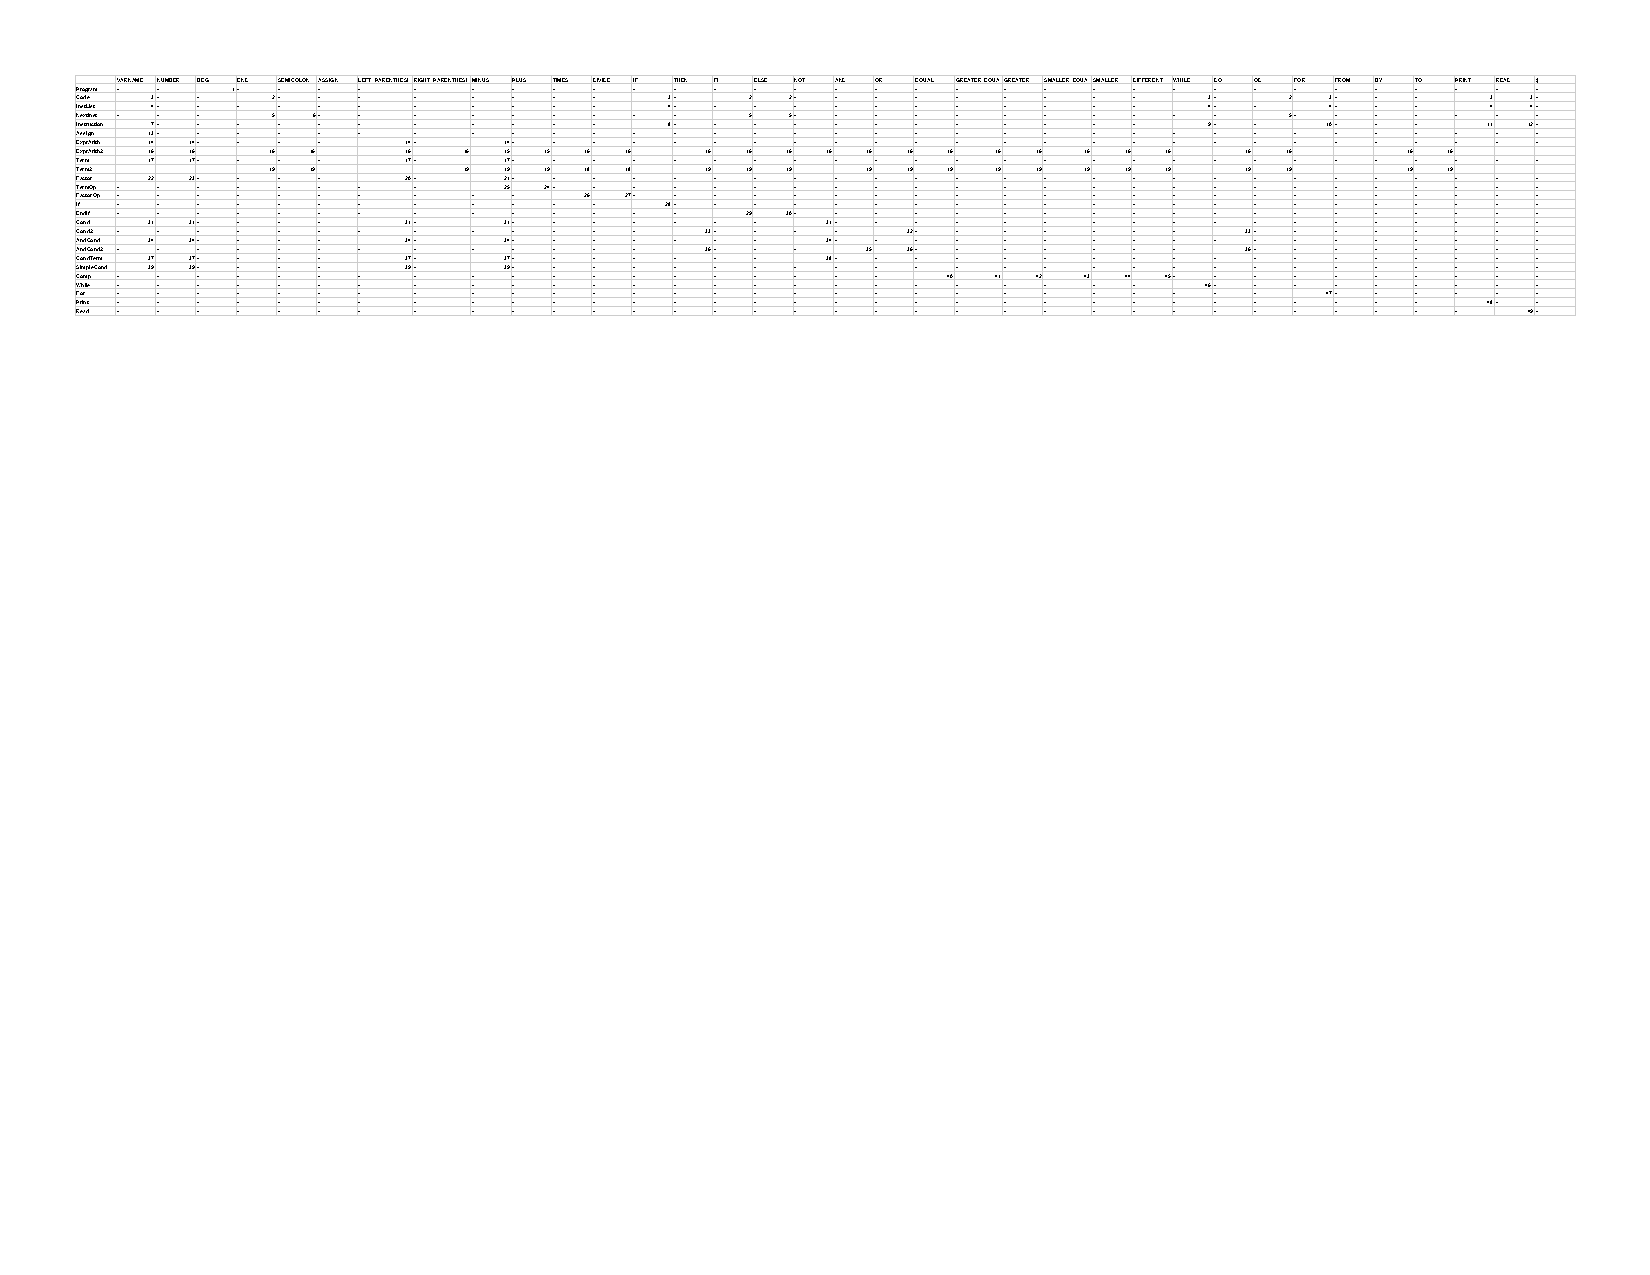
\includepdf[landscape=false]{TableauLL1.pdf}


\end{document}